
\begin{figure}[H]
\centering
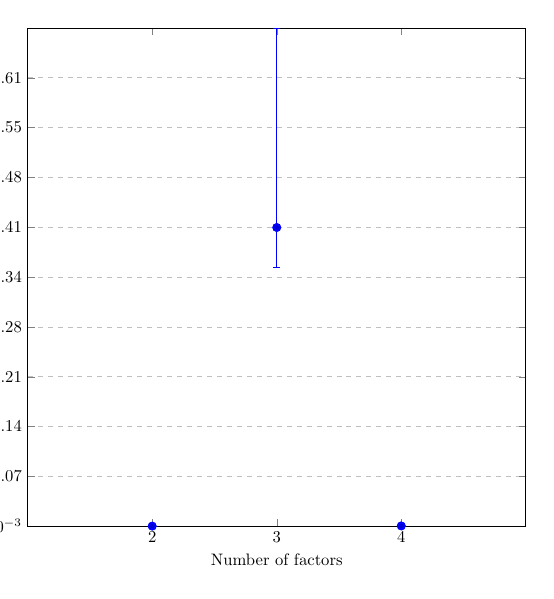
\begin{tikzpicture}[scale=0.6, trim axis left, trim axis right]
\begin{axis}[
    width=1\textwidth,
    height=1\textwidth,
    xlabel={Number of factors},
    ylabel={Time taken (s)},
    xmin=1.0, xmax=5.0,
    ymin=0.004221, ymax=60.681774,
    xticklabels={2, 3, 4},
    xtick={2, 3, 4},
    ytick={0.004221, 6.0719763, 12.1397316, 18.2074869, 24.2752422, 30.3429975, 36.4107528, 42.4785081, 48.5462634, 54.6140187},
    ymajorgrids=true,
    grid style=dashed,
]

\addplot+[
    blue,
    very thick,
    forget plot,
    only marks
    ]
    plot[
    very thick,
    error bars/.cd,
    y dir=plus,
    y explicit
    ]
    table[x=x,y=y,y error expr=\thisrow{y-max}] {
    x    y    y-max
    3	36.3810060769	24.3007679231
2	0.00736926	0.10174274
4	0.030567	0.001926

    };

\addplot+[
    blue,
    very thick,
    forget plot,
    only marks
    ]
    plot[
    very thick,
    error bars/.cd,
    y dir=plus,
    y explicit
    ]
    table[x=x,y=y,y error expr=\thisrow{y-min}] {
    x    y    y-min
    3	36.3810060769	-4.79636307692
2	0.00736926	-0.00314826
4	0.030567	-0.000277

    };

\end{axis}
\end{tikzpicture}
\vspace{-0.3cm}
\caption{FermatsFactorization medium primes }\label{fig:FermatsFactorizationmediumprimesfactors}
\end{figure}
